%---------------------------------------------------------------------
\begin{frame}{Back to context}

    \newbold{Grossman} model (1972) of demand for \textit{health}\\
    Health:
    \begin{itemize}
        \item Enters utility directly
        \item Is an investment
        \item Is an input in production of health and of productive time
    \end{itemize}
    \vspace{3mm}

    What about the demand for \sout{health} \textit{healthcare}?
    
\end{frame}
%---------------------------------------------------------------------
\begin{frame}{Some definitions}

    \newbold{Moral hazard}:\\
    \textit{Moral hazard is the change in an individual's behavior
    that occurs after entering into a contract because the individual
    does not bear the full consequences of their actions,
    typically due to imperfect observability or enforcement.}
    \vspace{5mm}

    \pause
    Two types of moral hazard:
    \begin{itemize}
        \item \newbold{Ex-ante moral hazard} {\color{gray} \small (Ehrlich and Becker, 1972)}: change in behavior \textit{before} an event occurs (e.g., risk-taking)
        \item \newbold{Ex-post moral hazard} {\color{gray} \small (Pauly, 1968)}: change in behavior \textit{after} an event occurs (e.g., consumption of care)
    \end{itemize}

\end{frame}
%-----------------------------
\begin{frame}{Examples of moral hazard}

    \begin{itemize}
        \item Banks engaging in excessive risk-taking knowing that the government will bail them out
        \item Individuals driving recklessly when they have car insurance
        \item More generous unemployment insurance may cause some workers to remain out of work longer
        \item \only<1>{Academic researchers slacking off after tenure} \only<2>{\newbold{Academic researchers slacking off after tenure}}
        \item Individuals consuming more healthcare when they have health insurance
    \end{itemize}
    
\end{frame}
%---------------------------------------------------------------------
\begin{frame}{Incentives in research? \textit{Hill \& Stein (2025)}}

    \vspace{-10mm}
    \begin{center}
        
\includegraphics[width=0.7\textwidth]{input/HillStein2025.pdf}
    \end{center}
    \vspace{-10mm}

    %Carolyn Stein's JMP.
    %Incentives to publish in molecular research: publish earlier to be the first, but lower quality research because not finished.

    % For me in tenure track, I need to publish as much as I can: I may undertake projects that less ambituous but easier to publish
    % Is it good for research? No, we don't want to skew knowledge toward the publication process.
    % Remedy? Tenure. Make me reveal that I am a motivated and productive researcher, and then shield me from publication incentives.

    {\small Hill, Ryan, and Carolyn Stein. \textit{``Race to the bottom: Competition and quality in science.''} The Quarterly Journal of Economics 140, no. 2 (2025): 1111-1185.}   
\end{frame}
%---------------------------------------------------------------------
\begin{frame}{Economists after tenure}

    \begin{center}
        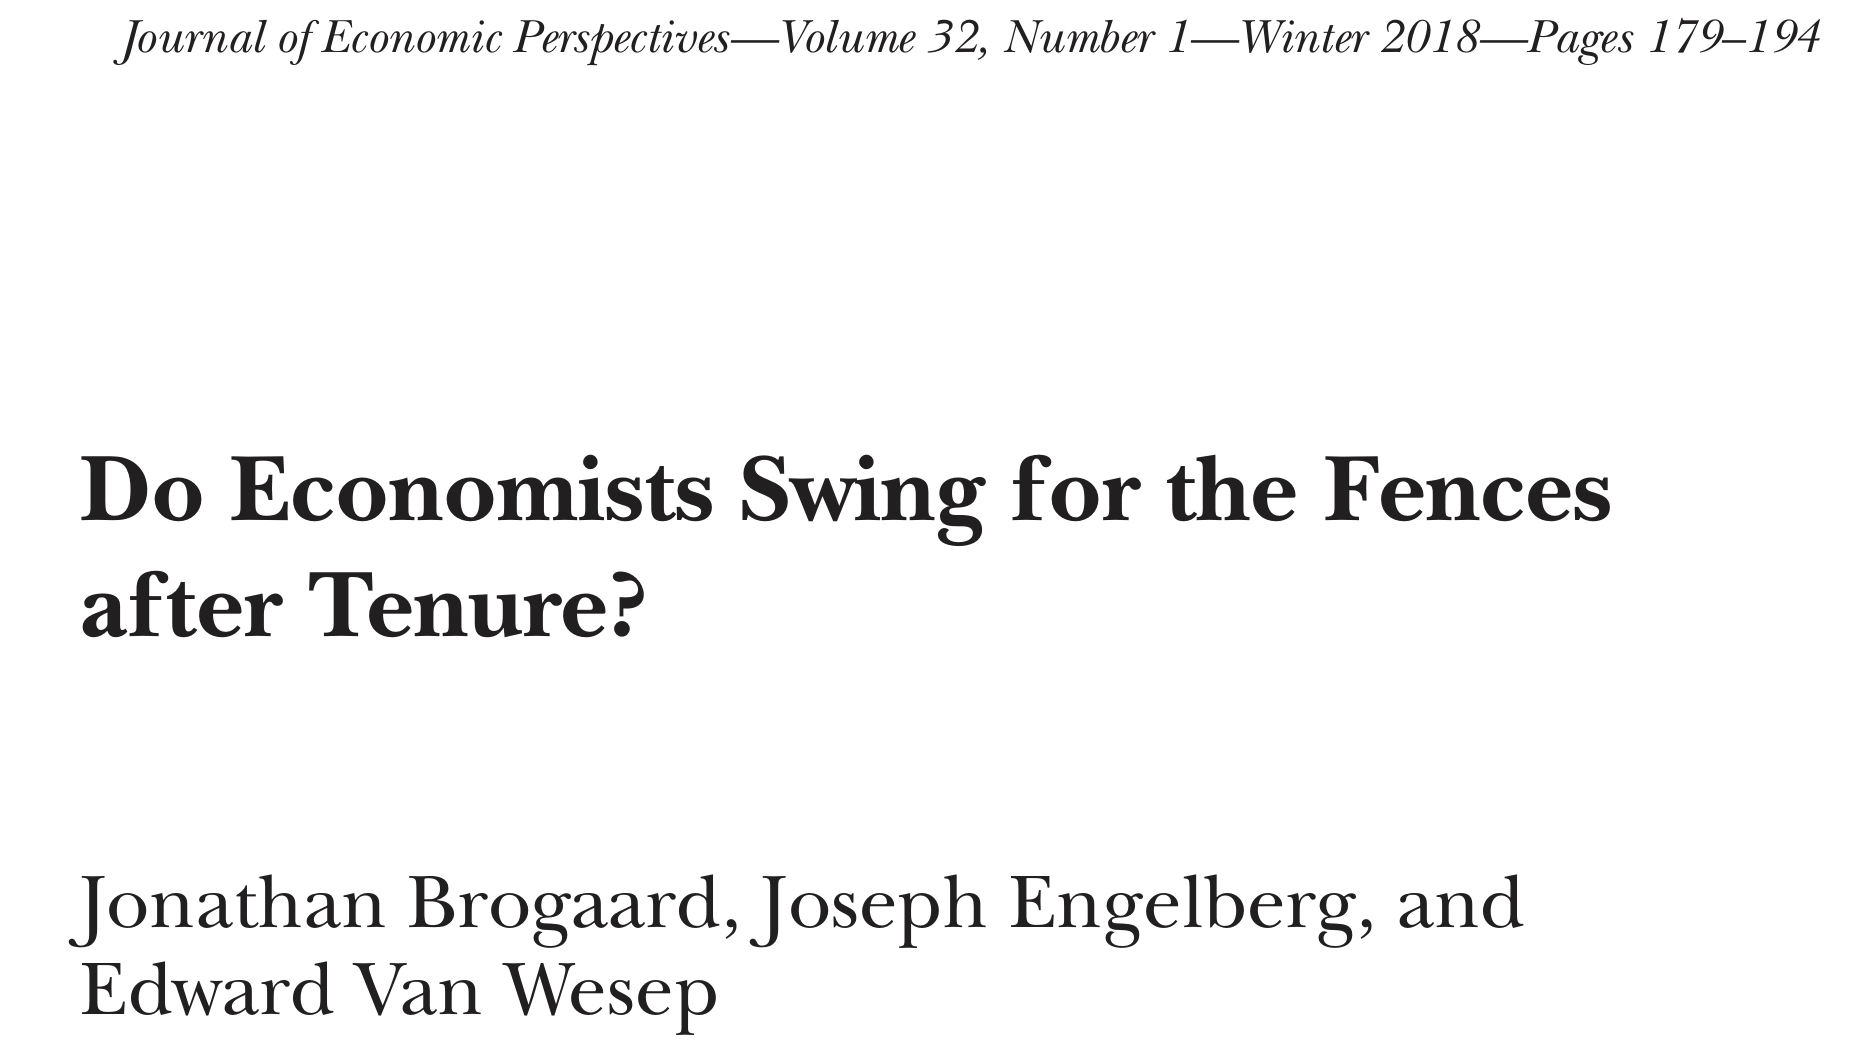
\includegraphics[width=0.7\textwidth]{input/academictenure_front.png}
    \end{center}

    { \small Source: \url{https://www.aeaweb.org/articles?id=10.1257/jep.32.1.179}}
    
\end{frame}
%---------------------------------------------------------------------
\begin{frame}{Economists after tenure}

    \begin{center}
        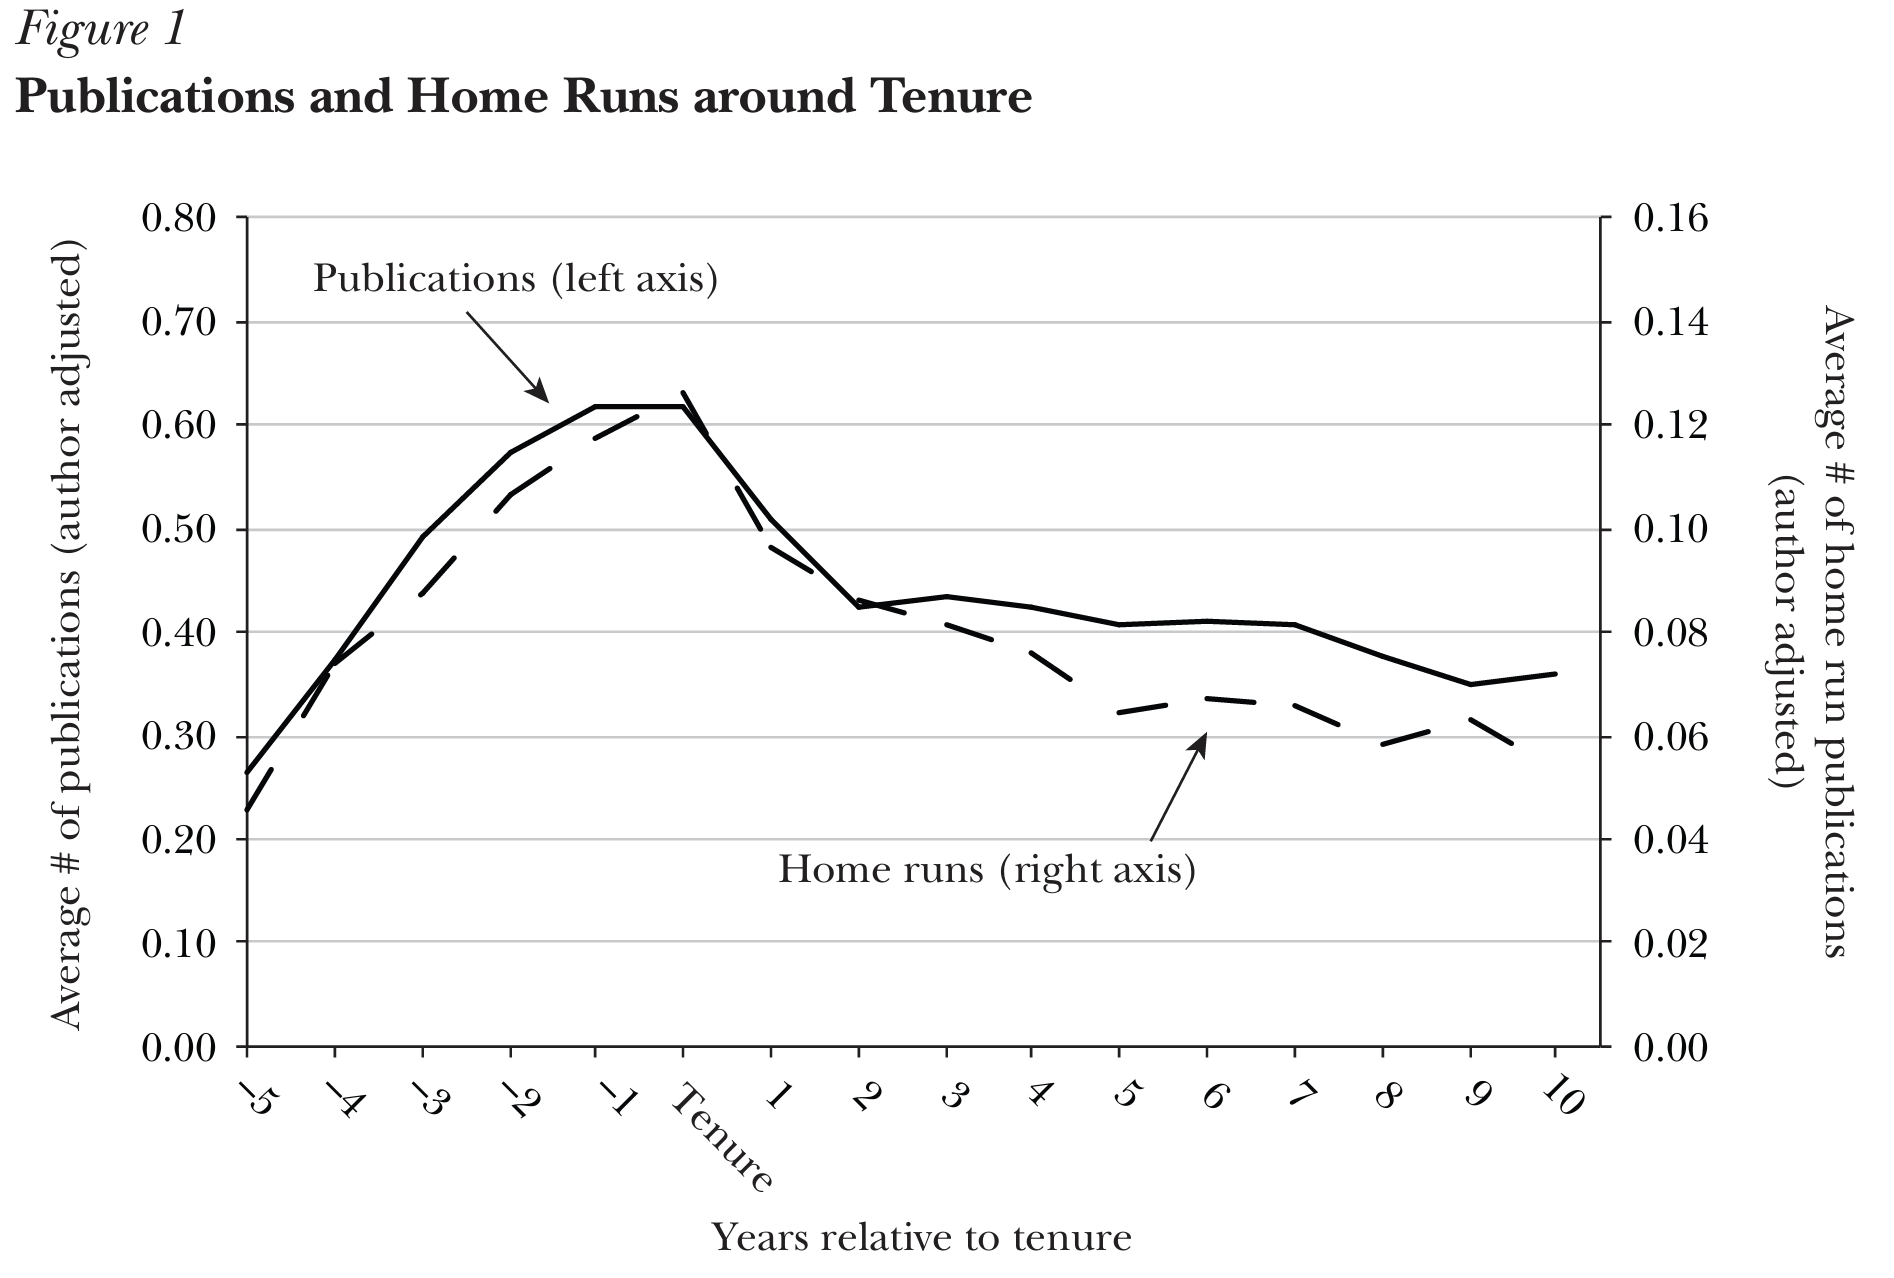
\includegraphics[width=0.7\textwidth]{input/academictenure_fig1.png}
    \end{center}
    
\end{frame}
%---------------------------------------------------------------------
\begin{frame}{Moral hazard in healthcare}

    Gaining insurance: price of healthcare is lower $\rightarrow$ individuals consume more healthcare\\
    \vspace{5mm}
    $\implies$ A rational response to an economic incentive?\\
    $\implies$ What is the price elasticity of demand for \textit{healthcare}?
    
\end{frame}
%---------------------------------------------------------------------
\begin{frame}{History of the term ``moral hazard''}

    Kenneth Arrow (1963):\textit{"the special economic problems of medical care can be explained by adaptations to uncertainty''}\\
    \vspace{2mm}

    Mark Pauly (1968): \textit{``in addition to the issues of risk and uncertainty,
    insurers also have to anticipate how consumers will respond to
    the changes in the price of healthcare caused by insurance''}
    \begin{itemize}
        \item Explains that the term ``moral hazard'' comes from medical insurance writers describing
        ``the hazard that arises from the failure of individuals
        who are or have been affected by insurance to uphold the accepted moral quantities''...
        \item ... but Pauly notes that ``the response of seeking more medical care with insurance ...
        is a result not of moral perfidy, but of rational economic behavior''
    \end{itemize}
    
\end{frame}
%---------------------------------------------------------------------
\begin{frame}{Reminder from last week}

    \newbold{Cost-sharing}: portion of medical bill that the patient is responsible for paying

        \centering
        \resizebox{0.7\textwidth}{!}{%
        \begin{tikzpicture}[>=Latex]
        
        \def\D{4.2}
        \def\M{9.2}
        \def\yD{3.2}
        \pgfmathsetmacro{\yMcalc}{\yD + 0.30*(\M-\D)}
        
        % Axes
        \draw[very thick,->] (0,0) -- (12,0);
        \draw[very thick,->] (0,0) -- (0,7.5);
        
        % Axis labels (FIXED)
        \node[below, font=\large, yshift = -18pt] at (6,0) {Dollars of health care expenses};
        \node[rotate=90, font=\large] at (-1.8,3.75) {Dollars of out-of-pocket expenses};
        
        % Vertical dashed lines
        \draw[dashed, thick] (\D,0) -- (\D,7.2);
        \draw[dashed, thick] (\M,0) -- (\M,7.2);
        
        % Labels on x-axis
        \node[below] at (\D,0) {\large 1,000};
        \node[below] at (\M,0) {\large max-OOP threshold};
        
        % OOP schedule
        \draw[very thick] (0,0) -- (\D,\yD);
        \draw[very thick] (\D,\yD) -- (\M,\yMcalc);
        \draw[very thick] (\M,\yMcalc) -- (12,\yMcalc);
        \draw[dashed, thick] (10.2,\yMcalc) -- (12,\yMcalc);
        
        % Slope annotations
        \node[rotate=36, yshift=7pt] at (2.2,1.9) {\large slope = 1};
        \node[rotate=17, yshift=5pt] at (6.8,4.2) {\large slope = 0.20};
        \node at (10.7,\yMcalc+0.35) {\large slope = 0};
        
        % Horizontal dashed line at OOP max = 3000
        \draw[dashed, gray, thick] (0,\yMcalc) -- (12,\yMcalc);
        \draw[gray, thick] (-0.15,\yMcalc) -- (0.15,\yMcalc);
        \node[left, gray, xshift=-4pt] at (0,\yMcalc) {\large 3{,}000};
    
        % Region braces
        \draw[decorate, decoration={brace, amplitude=6pt}]
            (0.6,6.0) -- (\D-0.25,6.0);
        \node[font=\large\itshape] at (\D/2,6.7) {deductible region};
        
        \draw[decorate, decoration={brace, amplitude=6pt}]
            (\D+0.25,6.0) -- (\M-0.25,6.0);
        \node[font=\large\itshape, align=center] at ({(\D+\M)/2},6.9)
            {20\% coinsurance\\region};
        
        \draw[decorate, decoration={brace, amplitude=6pt}]
            (\M+0.25,6.0) -- (11.6,6.0);
        \node[font=\large\itshape, align=center] at ({(\M+12)/2},6.9)
            {catastrophic \\care region};
        
        \end{tikzpicture}%
        }
\end{frame}
%---------------------------------------------------------------------
\begin{frame}{How to think about it?}

Insurer chooses:
\begin{enumerate}
    \item \newbold{Premium}: $p$
    \item \newbold{Coinsurance rate}: $s$
\end{enumerate}
\vspace{5mm}
Imagine the individual is sick and needs to pay \$25,000 in medical bills with probability 0.2.\\
$\implies$ What is the insurer's problem?\\
\pause
\begin{align*}
    &\max_{p,s} p - 0.2 * (1-s) * 25,000\\
    \text{such that}&\\
    & EU(\text{insured}) \geq EU(\text{not insured})
\end{align*}
% The insurer would have s= 0 (full insurance)
%if there was no moral hazard
%and would capture all consumer surplus with premium

\end{frame}
%---------------------------------------------------------------------
\begin{frame}{How to think about it?}

Moral hazard: $d > 0$\\
$\implies$ The individual would consume $\$25,000 \times \left( 1 + d \times s \right)$ in medical care if insured.\\
\vspace{5mm}
$\implies$ The insurer faces a trade-off:
\begin{itemize}
    \item Higher $s$ $\rightarrow$ less moral hazard $\rightarrow$ lower costs
    \item Higher $s$ $\rightarrow$ less attractive insurance $\rightarrow$ lower premium
\end{itemize}
\pause 
\vspace{5mm}
$\implies$ Is $d$ = 0? If not, how large is it?

\end{frame}
%----------------------------------------
\begin{frame}{}

    \begin{center}
        \Large \textcolor{maroon}{Back to basics of demand}
        \end{center}
\end{frame}
%---------------------------------------------------------------------
\begin{frame}{Demand}

    \begin{center}
        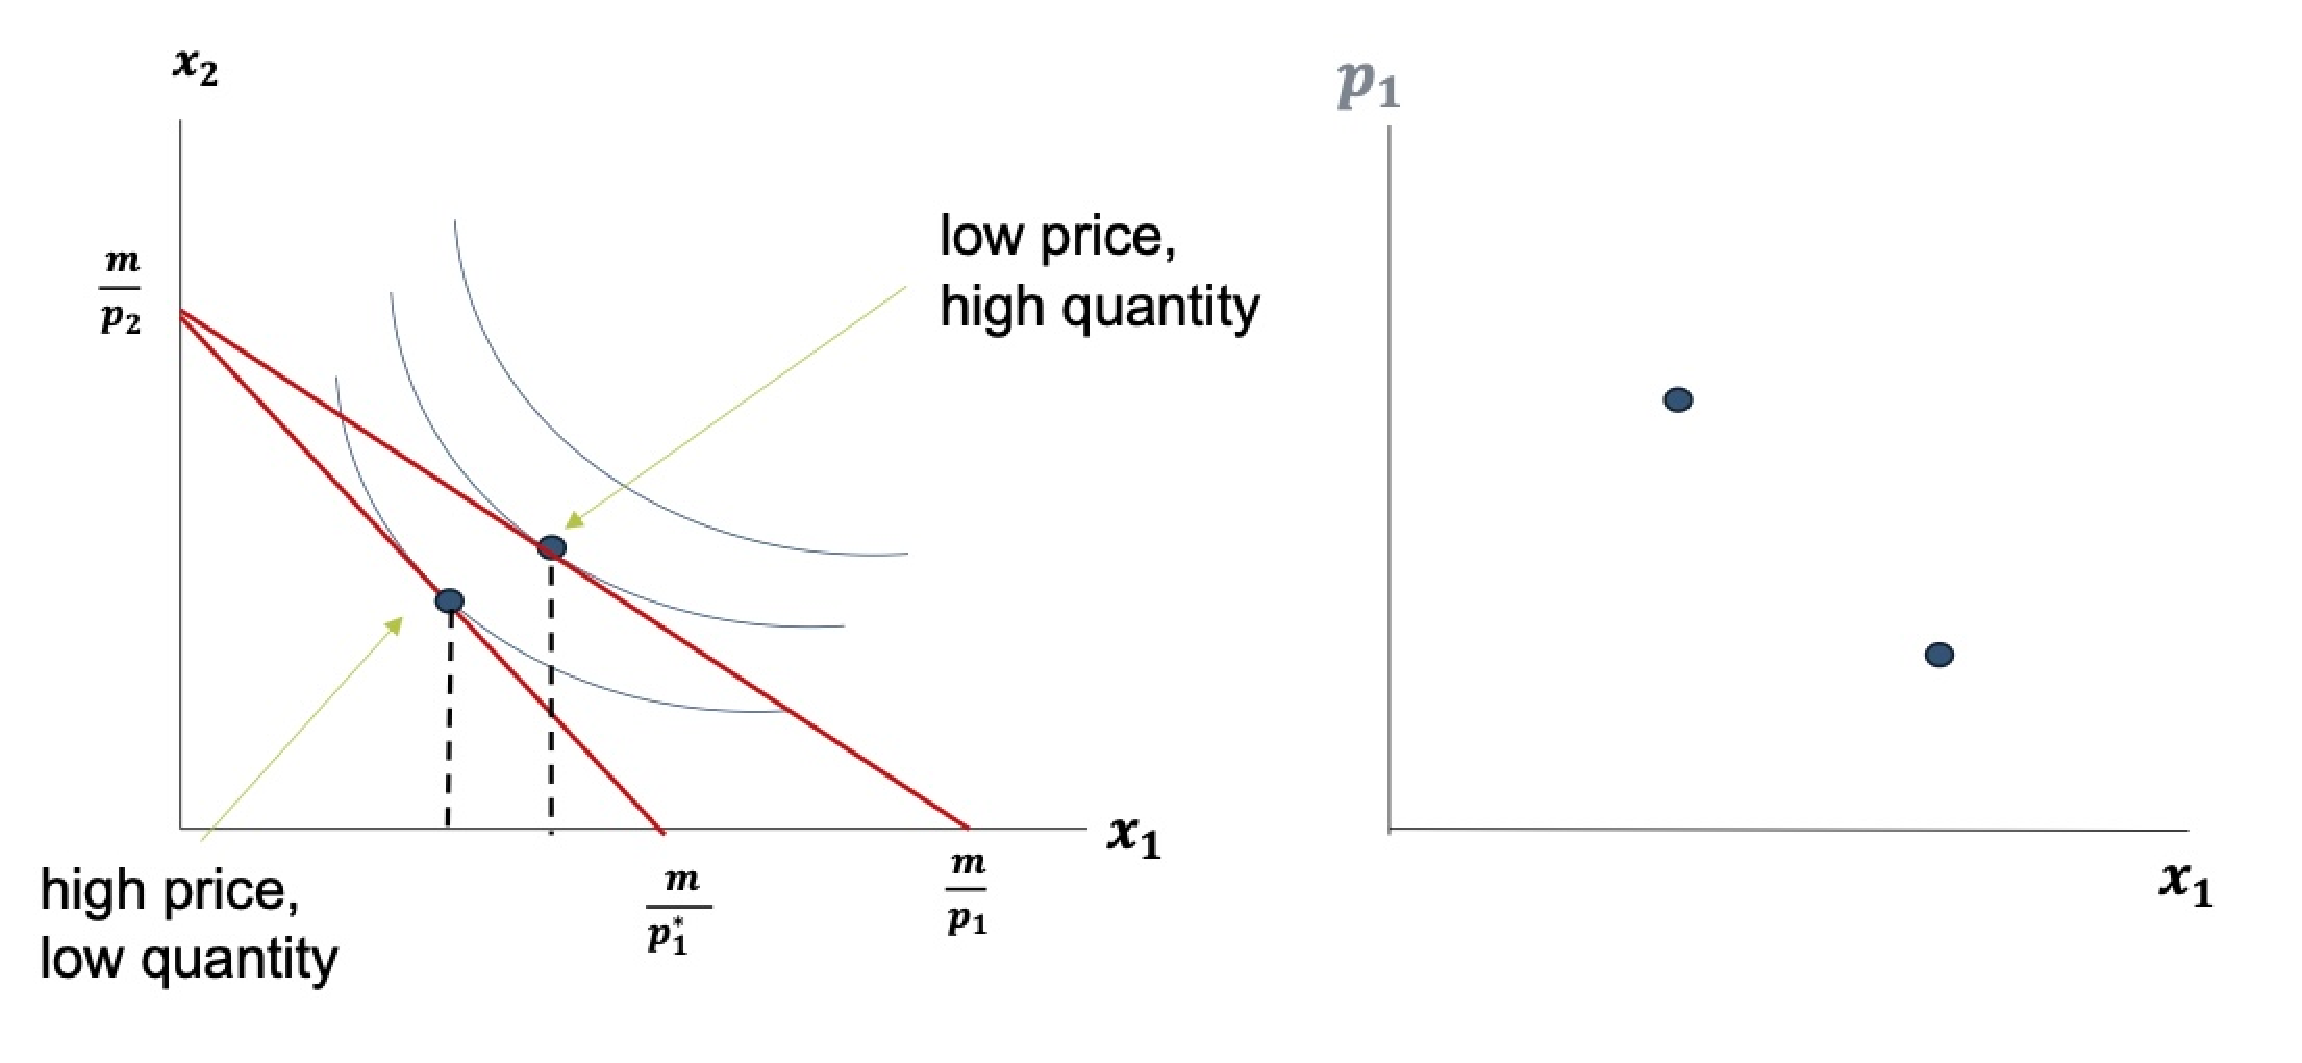
\includegraphics[width=0.95\textwidth]{input/indifference_curve_BC_7.pdf}
    \end{center}
 
 \end{frame}
%---------------------------------------------------------------------
\begin{frame}{Demand}
\begin{center}
    \begin{tikzpicture}[scale=0.9]

        %----- AXES -----
        \draw[thick] (0,0) -- (8,0) node[right, font=\large] {$x_1$};
        \draw[thick] (0,0) -- (0,6) node[above, font=\large] {$p_1$};
    
        %----- EXTENDED BLUE LINE TOUCHING BOTH AXES -----
        \draw[very thin, blue!50!black]
            (0,5.33) -- (7.5,0);
    
        %----- 7 DOTS ON THE BLUE LINE -----
        % Parametric representation of points between (0,5.33) and (7.5,0)
        \foreach \i in {0,...,6} {
            \pgfmathsetmacro{\t}{\i/6}
            \pgfmathsetmacro{\x}{0 + \t*(7.5 - 0)}
            \pgfmathsetmacro{\y}{5.33 + \t*(0 - 5.33)}
    
            \filldraw[
                fill=blue!50!black,
                draw=gray,
                line width=0.4pt
            ] (\x,\y) circle (3pt);
        }
    
    \end{tikzpicture}
\end{center}
 \textcolor{white}{$\implies$ This is the demand for good 1 $p_1(x_1)$.}
 \end{frame}

%---------------------------------------------------------------------
\begin{frame}{Move \textit{along} the demand}
        \begin{center}
            \begin{tikzpicture}[scale=0.7]

                %----- AXES -----
                \draw[thick] (0,0) -- (8,0) node[right, font=\large] {$x_1$};
                \draw[thick] (0,0) -- (0,6) node[above, font=\large] {$p_1$};
            
                %----- EXTENDED BLUE LINE TOUCHING BOTH AXES -----
                \draw[very thin, blue!50!black]
                    (0,5.33) -- (7.5,0);
            
                %----- TWO DOTS (upper and lower) -----
                % Upper dot at t = 0.2
                \pgfmathsetmacro{\tU}{0.2}
                \pgfmathsetmacro{\xU}{\tU*7.5}
                \pgfmathsetmacro{\yU}{5.33*(1 - \tU)}
                \filldraw[fill=blue!50!black, draw=gray, line width=0.4pt]
                    (\xU,\yU) circle (3pt);
            
                % Lower dot at t = 0.6
                \pgfmathsetmacro{\tL}{0.6}
                \pgfmathsetmacro{\xL}{\tL*7.5}
                \pgfmathsetmacro{\yL}{5.33*(1 - \tL)}
                \filldraw[fill=blue!50!black, draw=gray, line width=0.4pt]
                    (\xL,\yL) circle (3pt);
            
                %----- SHORTER PARALLEL ARROW ABOVE THE LINE -----
                % Shift upward and shorten horizontally by using t = 0.25 → 0.55
                \pgfmathsetmacro{\tA}{0.25}
                \pgfmathsetmacro{\xA}{\tA*7.5}
                \pgfmathsetmacro{\yA}{5.33*(1 - \tA)}
            
                \pgfmathsetmacro{\tB}{0.55}
                \pgfmathsetmacro{\xB}{\tB*7.5}
                \pgfmathsetmacro{\yB}{5.33*(1 - \tB)}
            
                % Vertical shift upward
                \pgfmathsetmacro{\shift}{0.35}
            
                \draw[->, thick, blue!50!black]
                    (\xA, \yA+\shift) -- (\xB, \yB+\shift);
            
        \end{tikzpicture}  
        \end{center}
  
\end{frame}
%---------------------------------------------------------------------
\begin{frame}{Demand elasticity}

    Demand elasticity $\epsilon$ (price elasticity of demand):
    \begin{align*}
        \epsilon = \frac{\overbrace{dQ/Q}^{\text{\% change in Q}}}{\underbrace{dP/P}_{\text{\% change in P}}}
         = \frac{dQ}{dP} \times \frac{P}{Q}
    \end{align*}
    \only<1>{\vspace{2mm}}
    \only<2>{\vspace{-2mm}}

    Example: Assume the demand is $P = 200 - 25 Q$. 
    \begin{enumerate}
        \item What is the expression for the elasticity? \only<2>{{\color{red} $\epsilon = - \frac{P}{25Q}$}}
        \item What is the elasticity at $P=100$? \only<2>{{\color{red} $\epsilon = -1$}}
        \item Use the elasticity to predict the change in demand from going to $P=100$ to $P=25$.
        \only<2>{{\color{red} 
        At $P=100$, $Q=4$ and $\epsilon = -1$.
        We have $-1 = \frac{dQ}{dP} \frac{P}{Q} = \frac{dQ}{-(100-25)} \frac{100}{4}$.\\
        Solving for $dQ$ gives $dQ = 3$ and $Q' = 4+3 =7$.}}
    \end{enumerate}
\end{frame}
%--------------------------------------------------------------------
\begin{frame}{Demand elasticity}

\begin{center}
    \begin{tikzpicture}[scale=0.9, line cap=round, line join=round]

        % ---------------- Parameters ----------------
        \def\xmax{10}
        \def\ymax{7}
        \def\Pint{6.3}    % price intercept P
        \def\Qint{9.6}    % quantity intercept Q
      
        % ---------------- Coordinates ----------------
        \coordinate (O)   at (0,0);
        \coordinate (X)   at (\xmax,0);
        \coordinate (Y)   at (0,\ymax);
      
        % Demand intercepts
        \coordinate (P0)  at (0,\Pint);                 
        \coordinate (Q0)  at (\Qint,0);                  
      
        % Unit elasticity point
        \coordinate (E)   at ({0.5*\Qint},{0.5*\Pint});  
      
        % Slightly offset points around E
        \coordinate (Eup) at ($(P0)!0.97!(E)$);
        \coordinate (Edn) at ($(Q0)!0.97!(E)$);
      
        % ---------------- Axes ----------------
        \draw[very thick,->] (O) -- (X);
        \draw[very thick,->] (O) -- (Y);
      
        % Axis labels (tuned positions)
        \node[font=\bfseries\Large] at (\xmax,-0.55) {$Q$};       % x-axis label under arrow
        \node[font=\bfseries\Large] at (-0.45,\ymax-0.15) {$P$}; % y-axis label near arrow
      
        % Mark P/2 on y-axis
        \node[font=\bfseries\Large] at (-0.85,{0.5*\Pint}) {$P/2$};
      
        % ---------------- Demand curve ----------------
        \draw[very thick] (P0) -- (Q0);
      
        % ---------------- Dashed line at P/2 ----------------
        \draw[dashed, thick] (0,{0.5*\Pint}) -- (E);
      
        % ---------------- epsilon = -1 point ----------------
        \fill (E) circle (3pt);
      
        \node[font=\bfseries\Large] (epslab) at ($(E)+(2.1,1.4)$) {$\varepsilon=-1$};
        \draw[->, thick] (epslab.south west) -- ($(E)+(0.15,0.15)$);
      
        % ---------------- Braces + region labels ----------------
        % Elastic
        \draw[decorate, decoration={brace, amplitude=10pt, raise=10pt}]
          (P0) -- (Eup)
          node[midway,
               xshift=80pt,
               yshift=34pt,
               font=\bfseries\Large]
          {$-\infty<\varepsilon<-1$ (Elastic)};
      
        % Inelastic
        \draw[decorate, decoration={brace, amplitude=10pt, raise=10pt}]
          (Edn) -- (Q0)
          node[midway,
               xshift=75pt,
               yshift=34pt,
               font=\bfseries\Large]
          {$-1<\varepsilon\le 0$ (Inelastic)};
      
      \end{tikzpicture}      
    \end{center}
      
\end{frame}
%--------------------------------------------------------------------
\begin{frame}{Demand elasticity: some examples}

    \begin{center}
        \footnotesize
        \begin{table}[htbp]
            \centering
            \caption{Price Elasticity of Demand}
            \label{tab:price_elasticity}
            \begin{tabular}{l c}
            \hline
            \textbf{Good} & $\lvert \varepsilon \rvert$ \\
            \hline
            Airline travel   & 2.4  \\
            Restaurant meals & 2.3  \\
            Housing          & 1.2  \\
            Movies           & 0.9  \\
            Gasoline (LR)    & 0.7  \\
            Coffee           & 0.25 \\
            Automobiles      & 0.2  \\
            Gasoline (SR)    & 0.2  \\
            Outpatient care  & 0.17 \\
            Inpatient care   & 0.14 \\
            \hline
            \end{tabular}
            \end{table}              
        \end{center}
          
        %Comes fron Noto's slides
    \end{frame}
%--------------------------------------------------------------------
\begin{frame}{}

    \begin{center}
        \Large \textcolor{maroon}{Is the demand for healthcare different than other goods?}
        \end{center}
\end{frame}
%---------------------------------------------------------------------
\begin{frame}{What is cost-sharing?}

    \newbold{Cost-sharing}: portion of medical bill that the patient is responsible for paying
    \vspace{5mm}

    Demand slopes \newbold{down}
    \begin{enumerate}
        \item Is this true in healthcare? \only<2>{\newbold{Late 70s: was a debate.}}
        \item If so, to what extent? \only<2-3>{\textit{Elasticity of healthcare demand}}
        \item What does this mean for insurance?
    \end{enumerate}
\end{frame}
%---------------------------------------------------------------------
\begin{frame}{The \newbold{RAND health insurance experiment}}

    \textcolor{gray}{\textit{Back to the late 70s in California...}}
    \begin{center}
    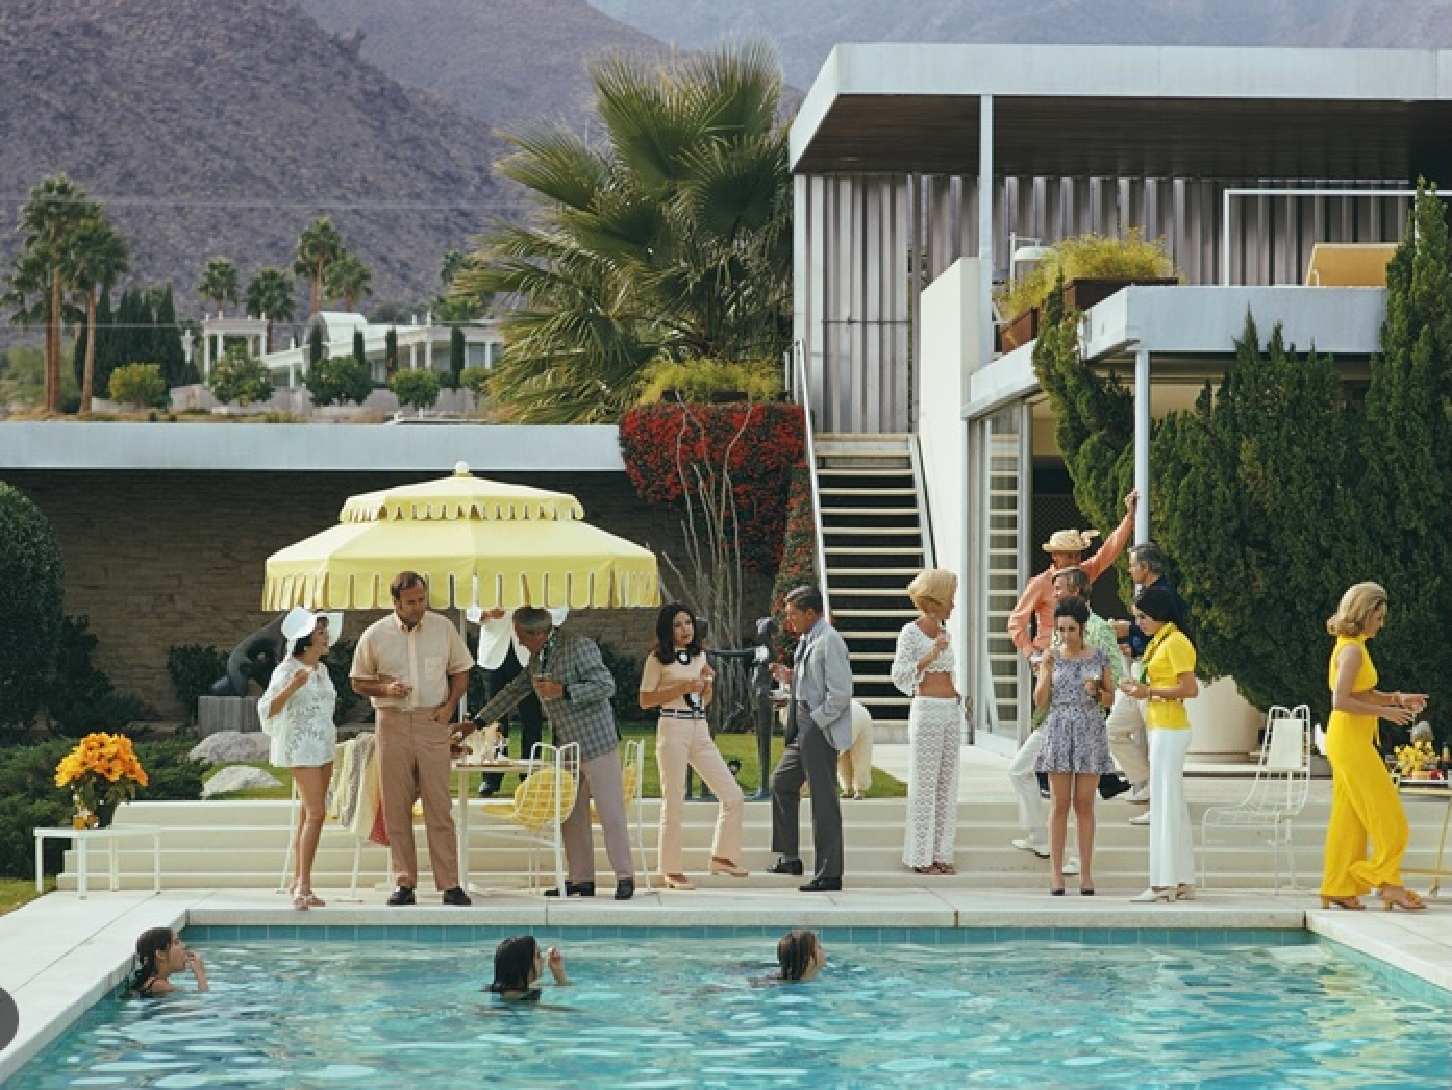
\includegraphics[width=0.5\textwidth]{input/CA_70s.pdf}
    \end{center}

\end{frame}
%---------------------------------------------------------------------
\begin{frame}{Reading: the RAND health insurance experiment}

    \begin{center}
        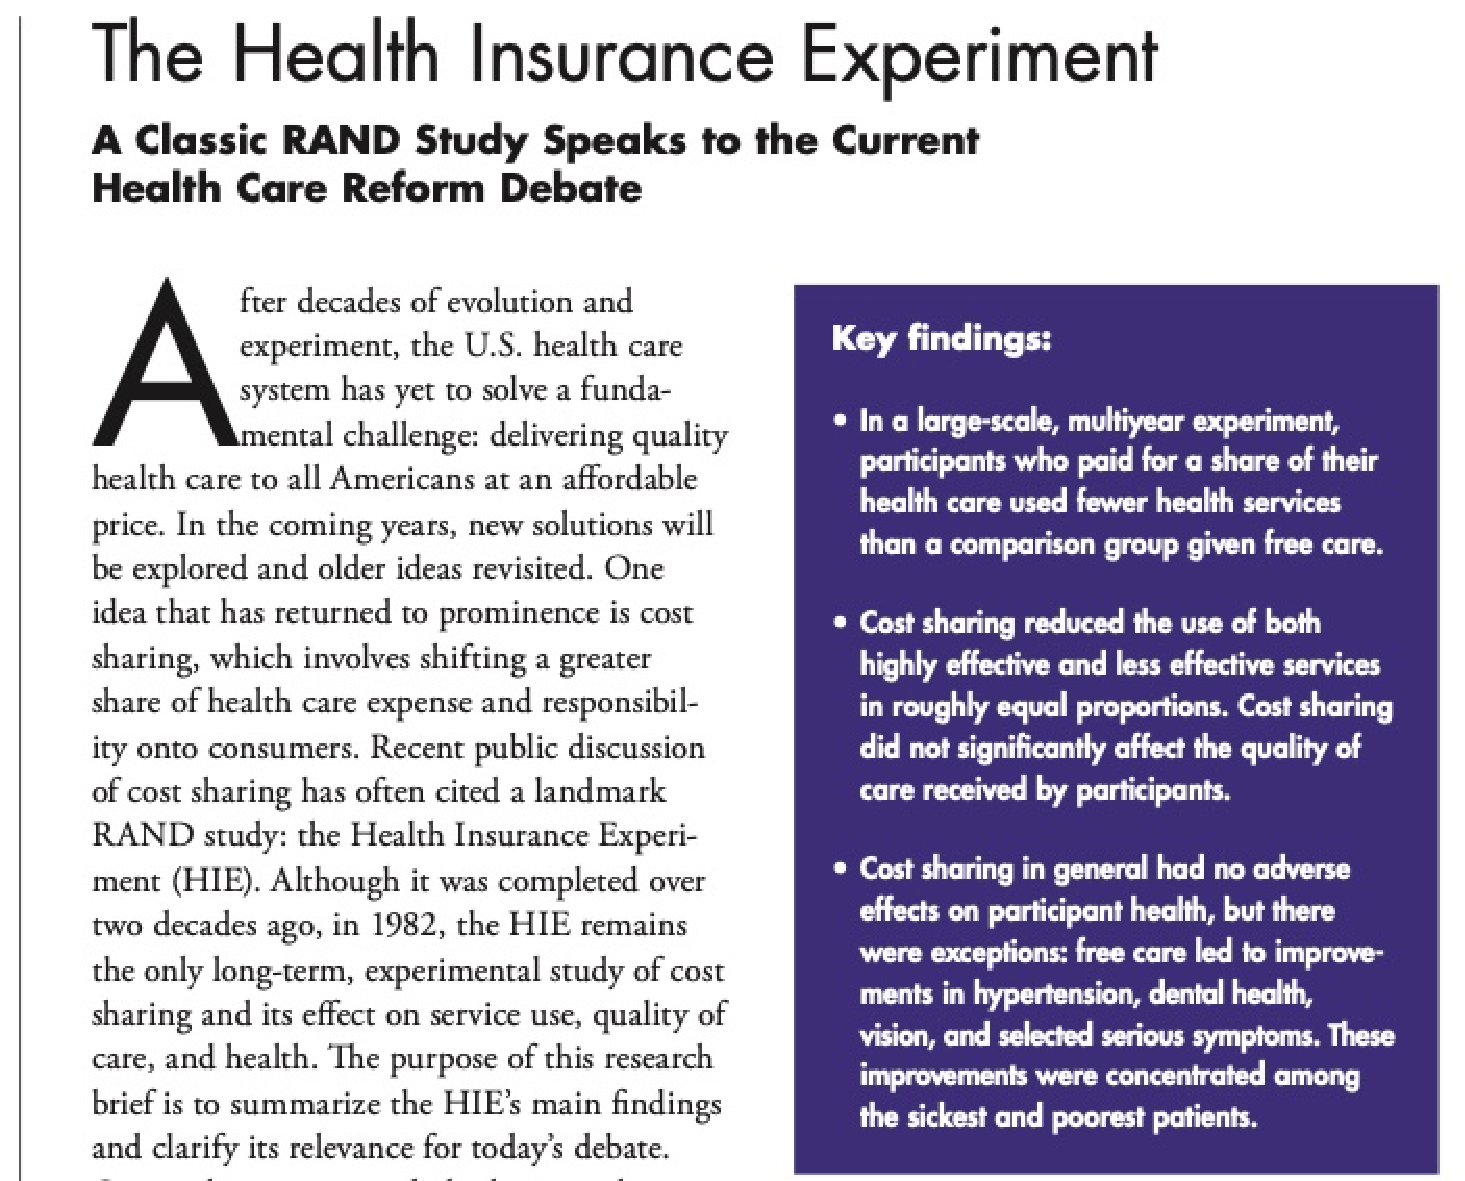
\includegraphics[width=0.6\textwidth]{input/RAND_frontarticle.pdf}
    \end{center}
\end{frame}
%---------------------------------------------------------------------
\begin{frame}{The \newbold{RAND health insurance experiment}}

    The \newbold{RAND health insurance experiment}
        \begin{itemize}
            \item Joe Newhouse (PI) at the RAND corporation
            \item 1974-1981: randomize $\approx$ 2,000 families into plans with \newbold{different cost-sharing}
            \item Duration of experiment: 3-5 years
            \item 6 enrollment sites
            \item Outcomes of interest: health spending and health
        \end{itemize}
        \vspace{3mm}
  
        
    A pioneering study
        \begin{itemize}
            \item One of the largest experiments (\$300 million in 2011 dollars)
            \item Screening questionnaires
            \item The experiment \textbf{acts as your insurer}
        \end{itemize}
        %pioneers: pioneers in what was then relatively novel territory for the social sciences, 
        %both in the conduct and analysis of randomized experiments and in the economic analysis of moral hazard in the context of health insurance. 
        %Still "gold standard" evidence for predicting the likely impact of health insurance reforms on medical spending
        %enormous influence on state and federal policy makers when thinking about policy interventions to reduce spending in healthcare

\end{frame}
%---------------------------------------------------------------------
\begin{frame}{The \newbold{RAND health insurance experiment}}

    \begin{center}
        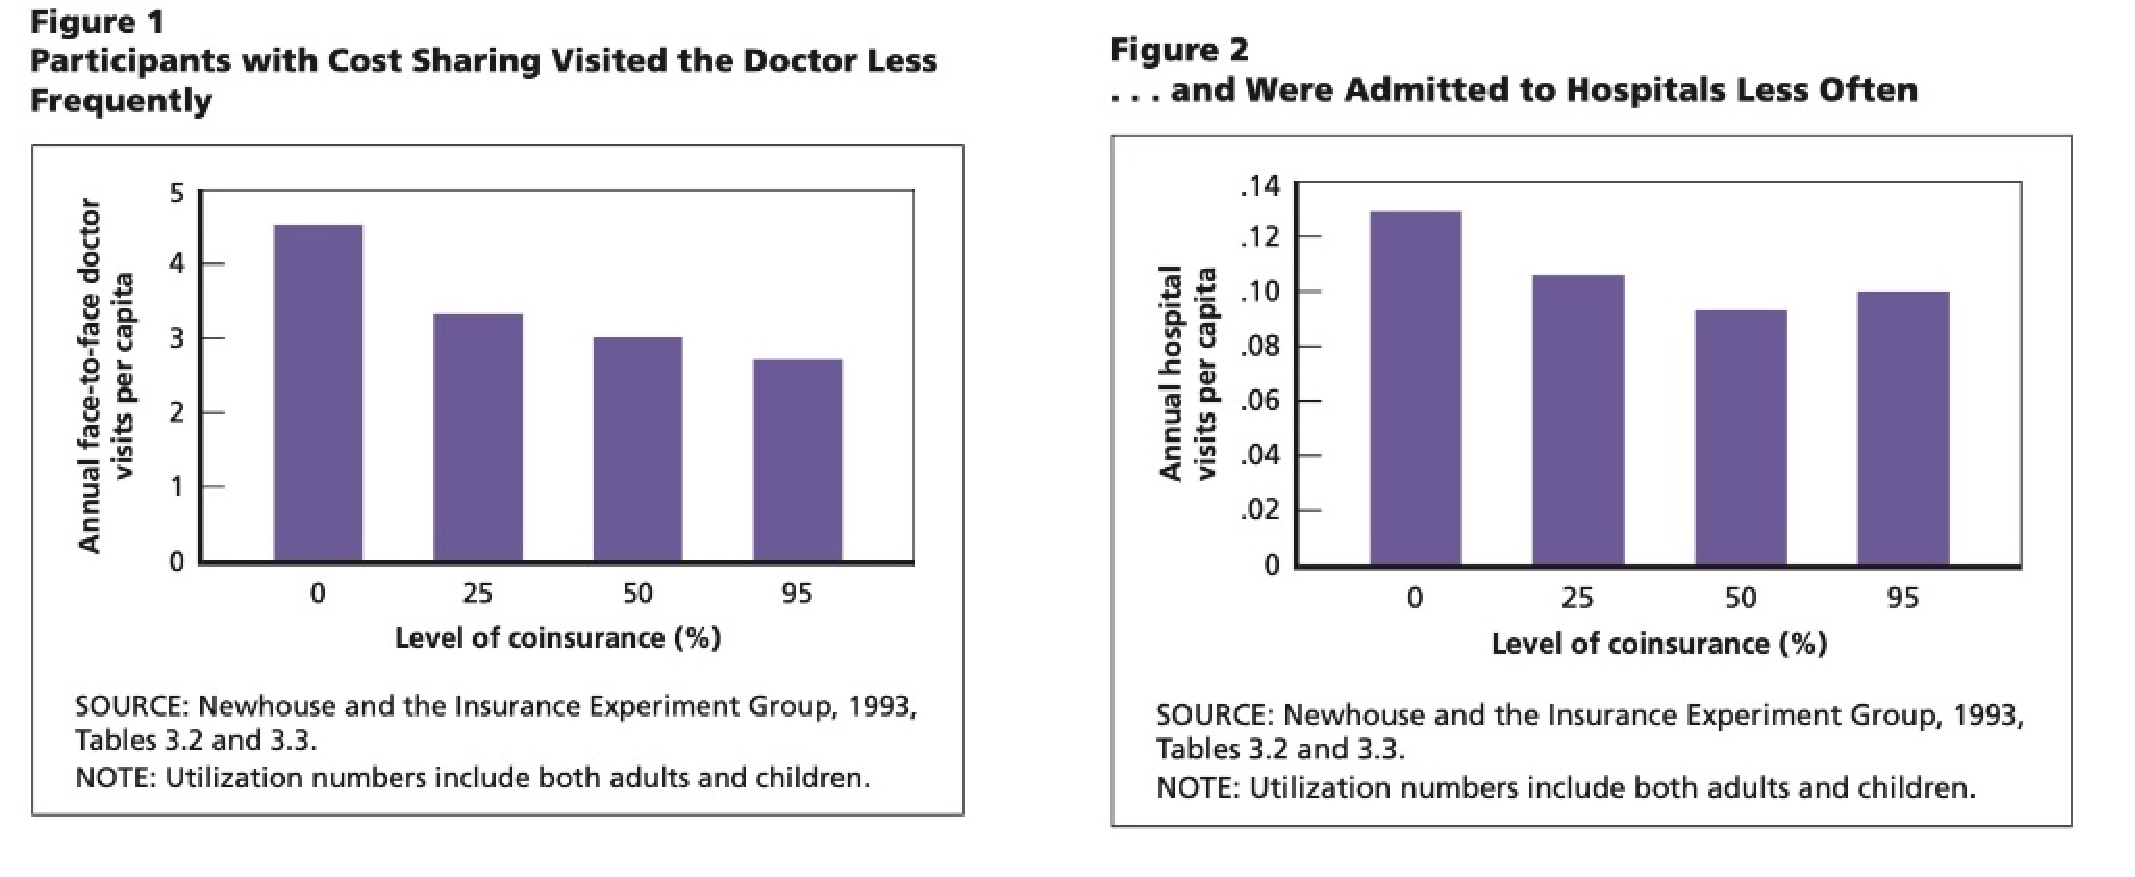
\includegraphics[width=1\textwidth]{input/RAND_fig1and2.pdf}
    \end{center}

\end{frame}
%---------------------------------------------------------------------
\begin{frame}{The \newbold{RAND health insurance experiment}}

    \begin{center}
        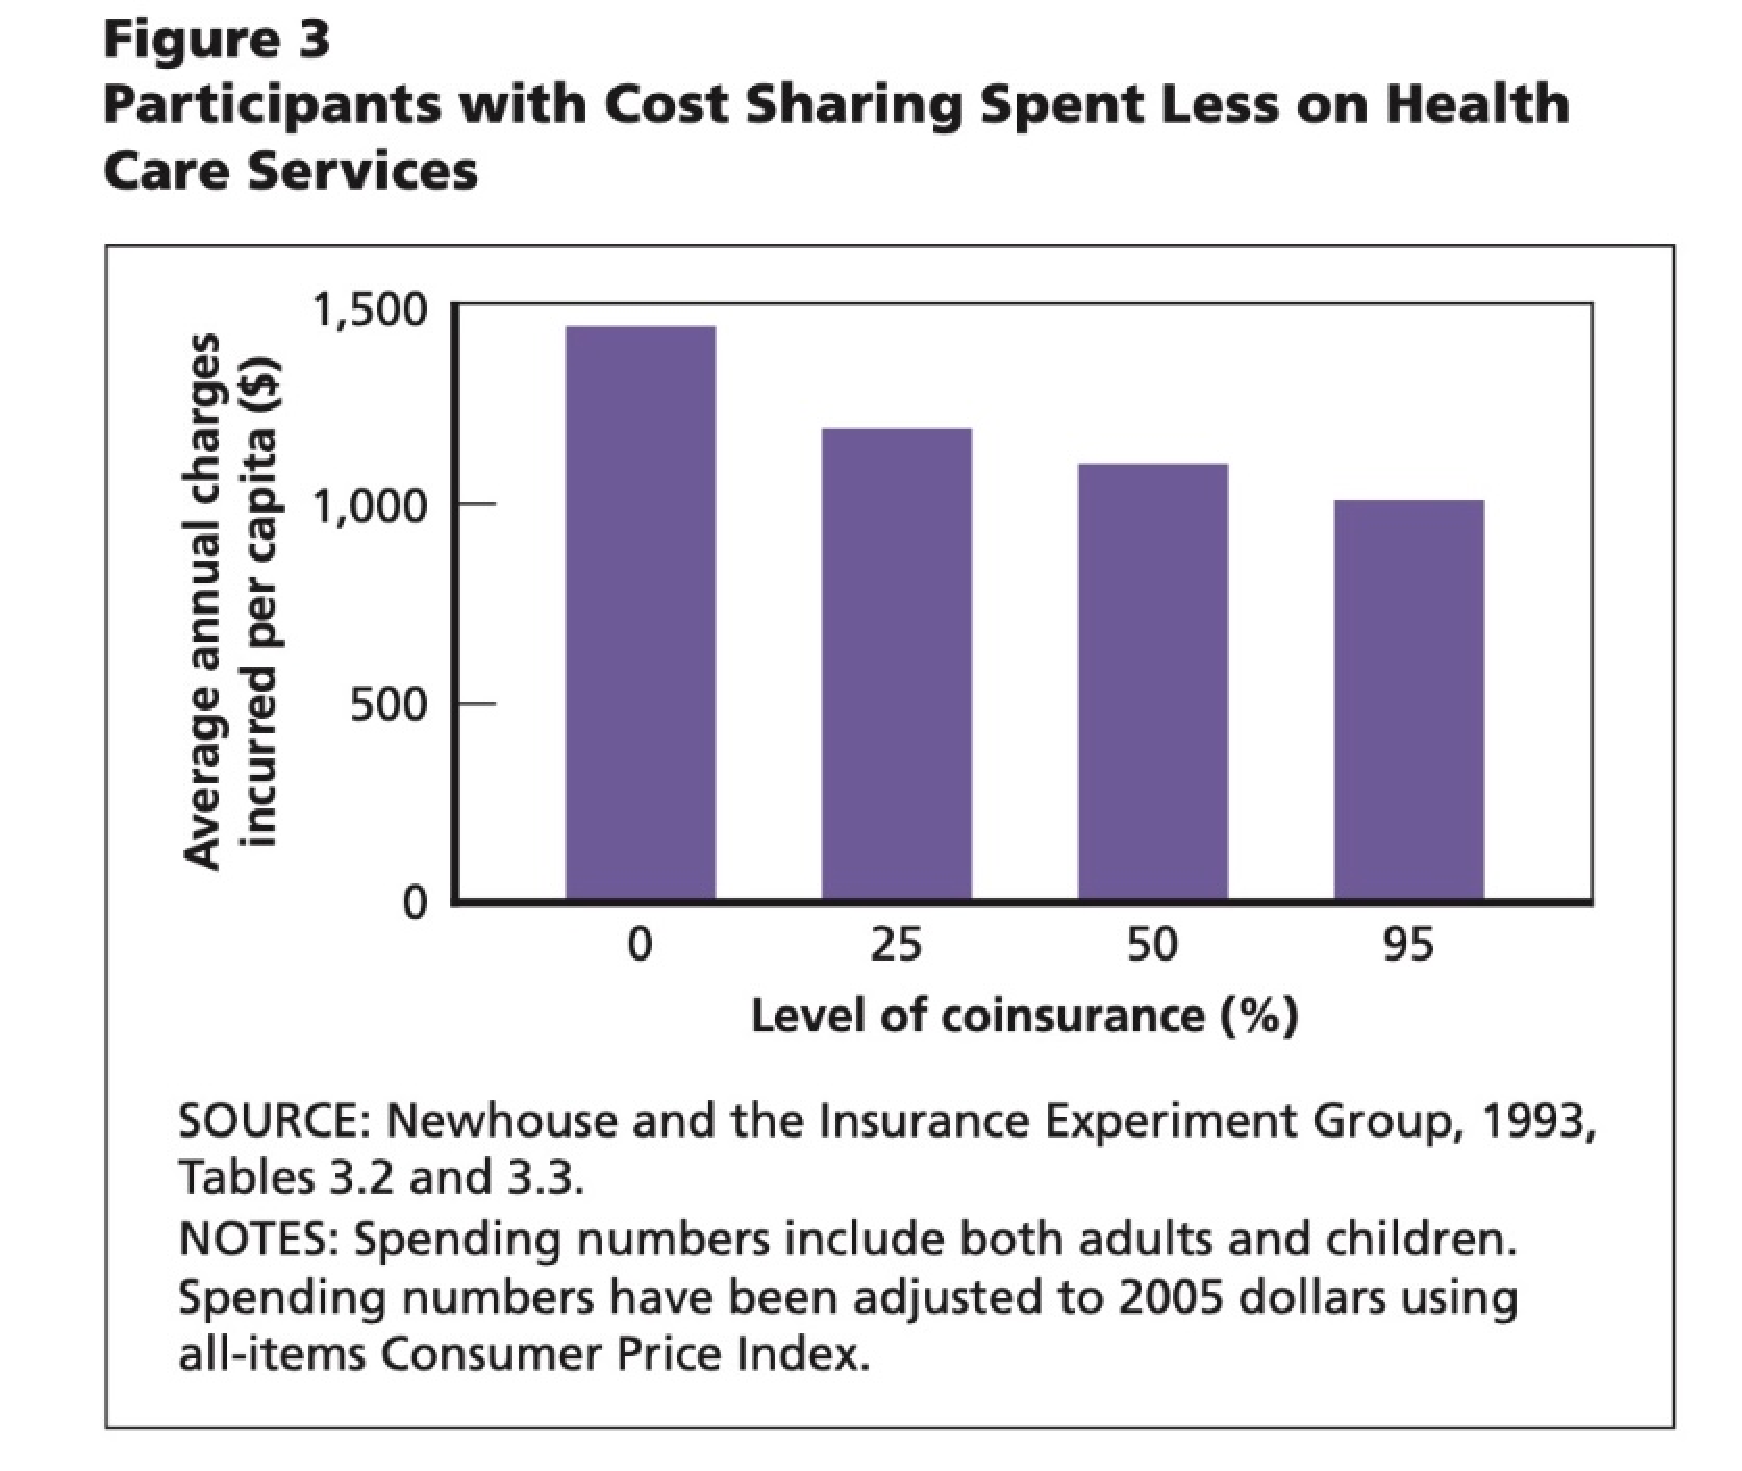
\includegraphics[width=0.6\textwidth]{input/RAND_figure3.pdf}
    \end{center}

\end{frame}
%---------------------------------------------------------------------
\begin{frame}{Which kind of care is consumed less?}

    \only<1>{
    \begin{center}
        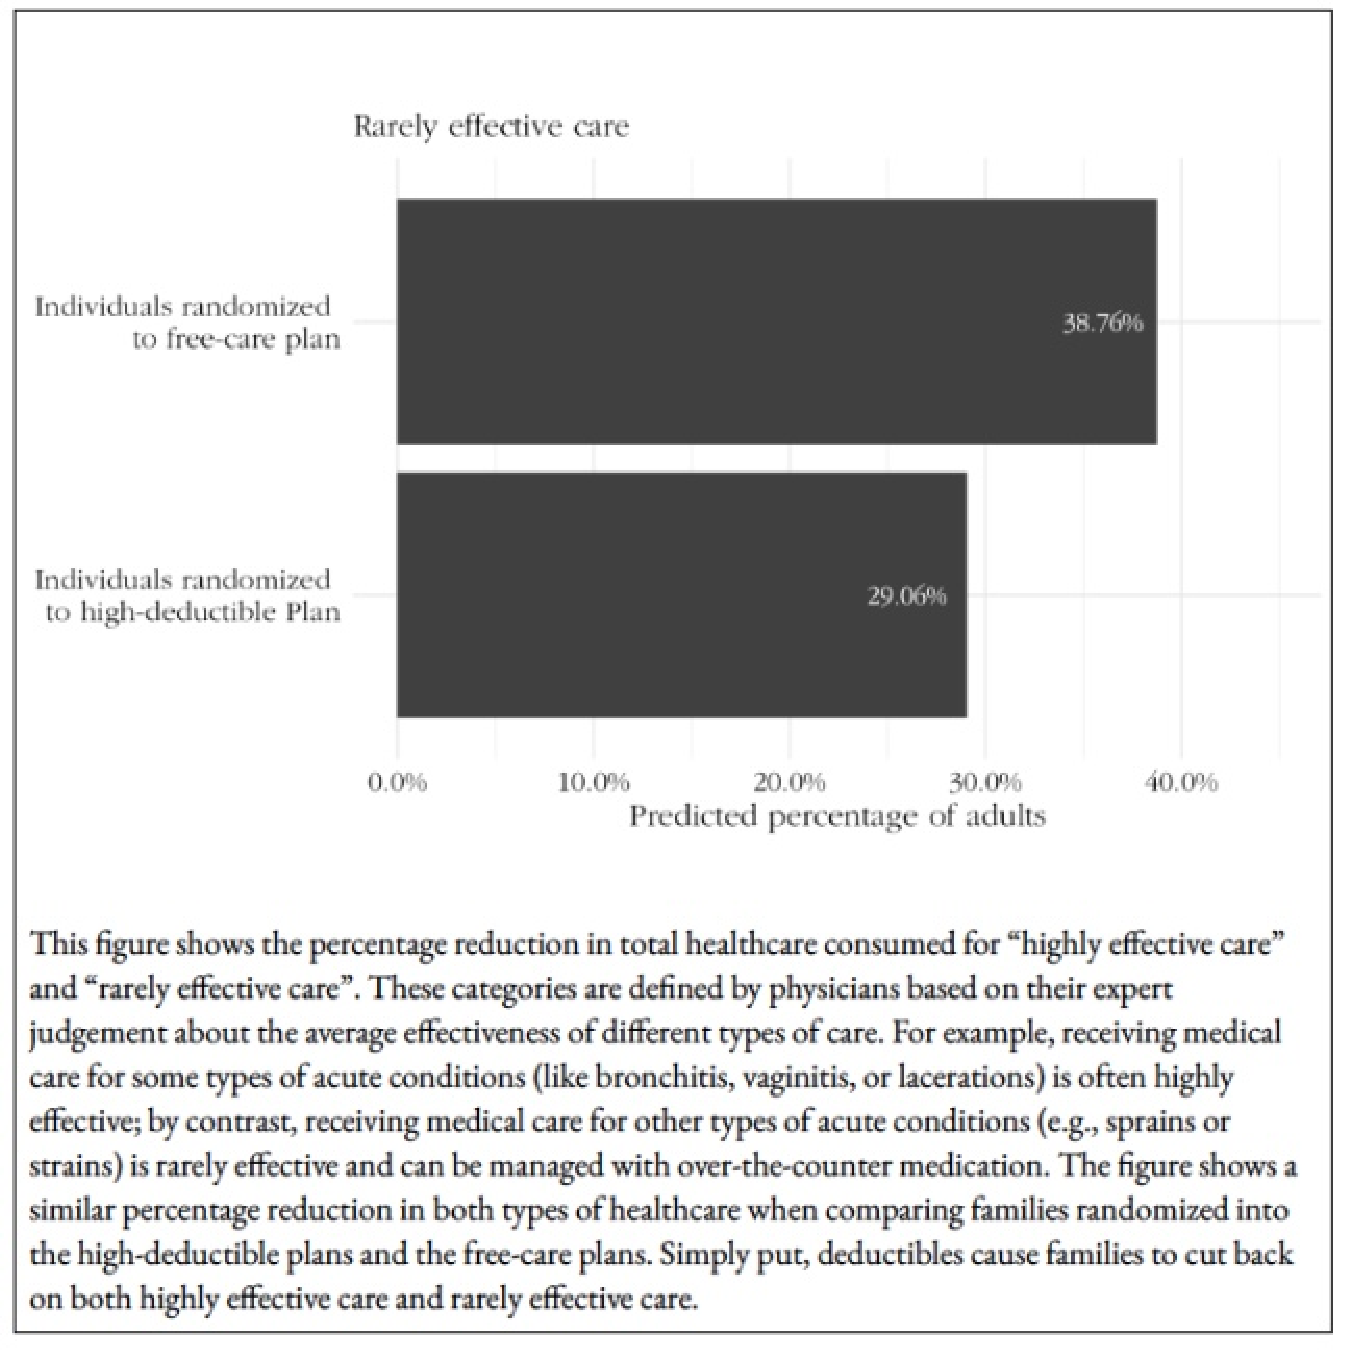
\includegraphics[width=0.45\textwidth]{input/RAND_rarelyeffectivecare.pdf}
    \end{center}
    \textcolor{white}{$\implies$ Which care is cut? Both ``rarely effective'' and ``effective'' care.}
    } \only<2>{
        \begin{center}
            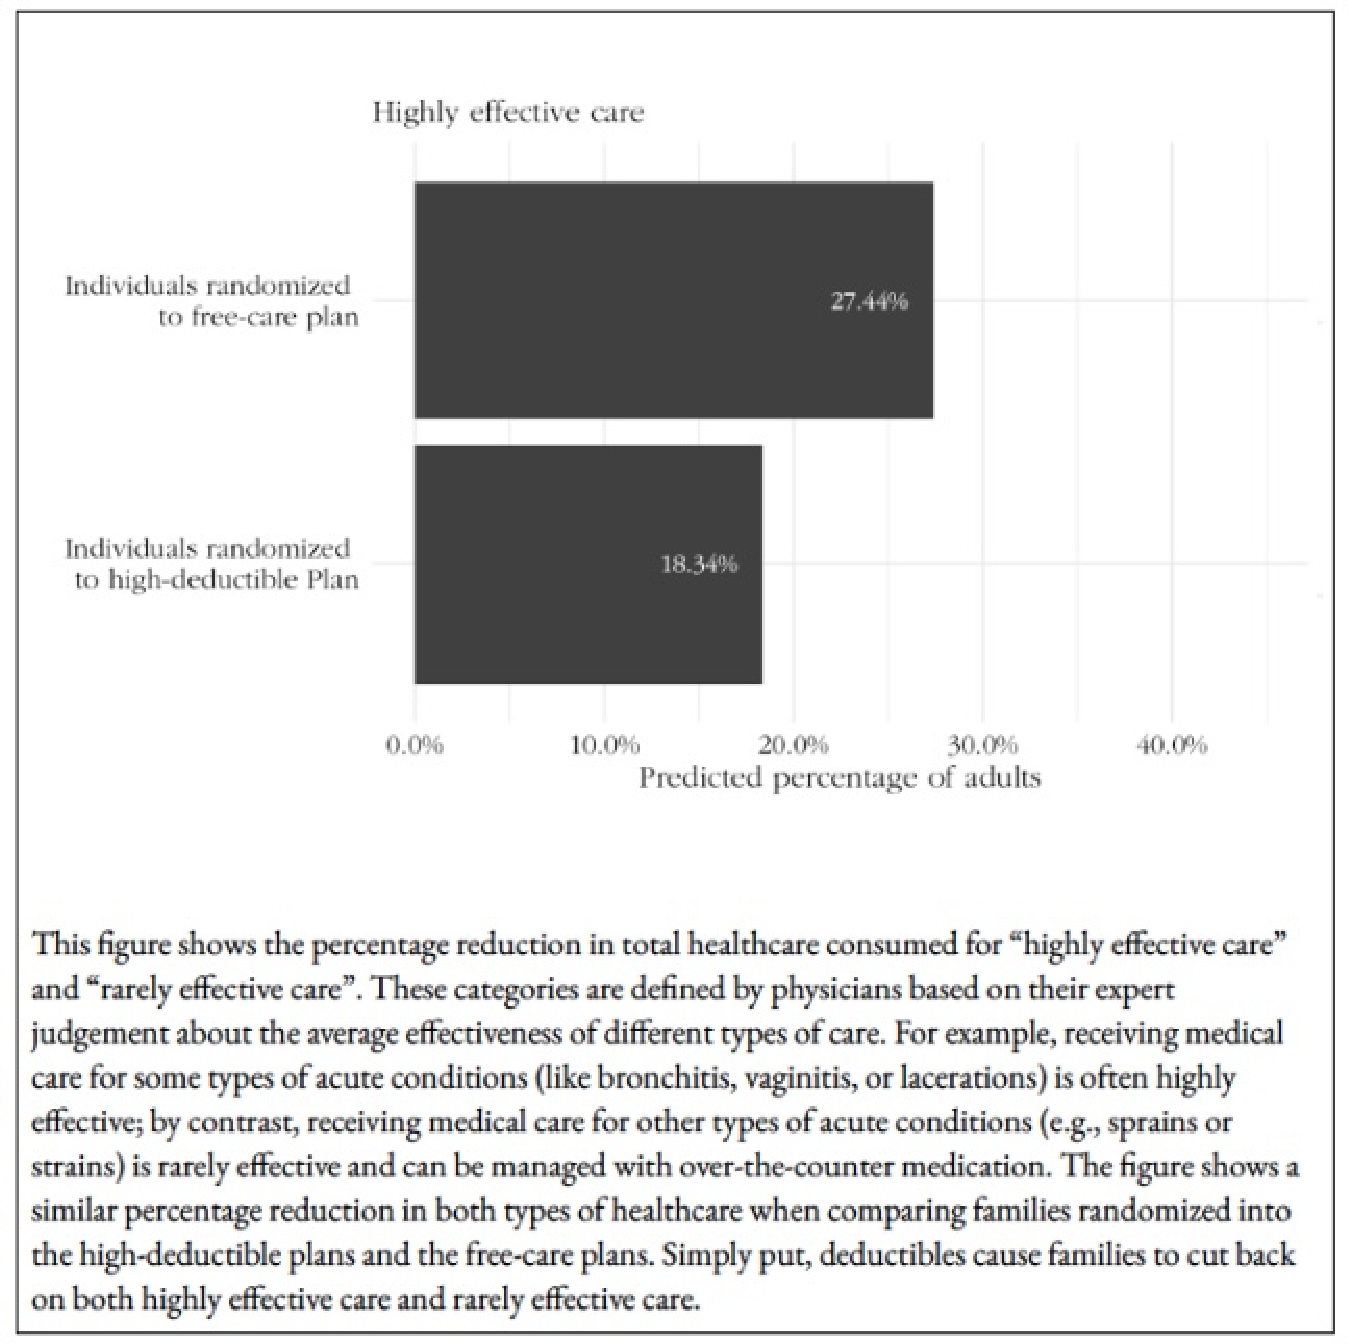
\includegraphics[width=0.45\textwidth]{input/RAND_effectivecare.pdf}
        \end{center}
        \textcolor{white}{$\implies$ Which care is cut? Both ``rarely effective'' and ``effective'' care.}
        }
    \only<3>{
        \begin{center}
            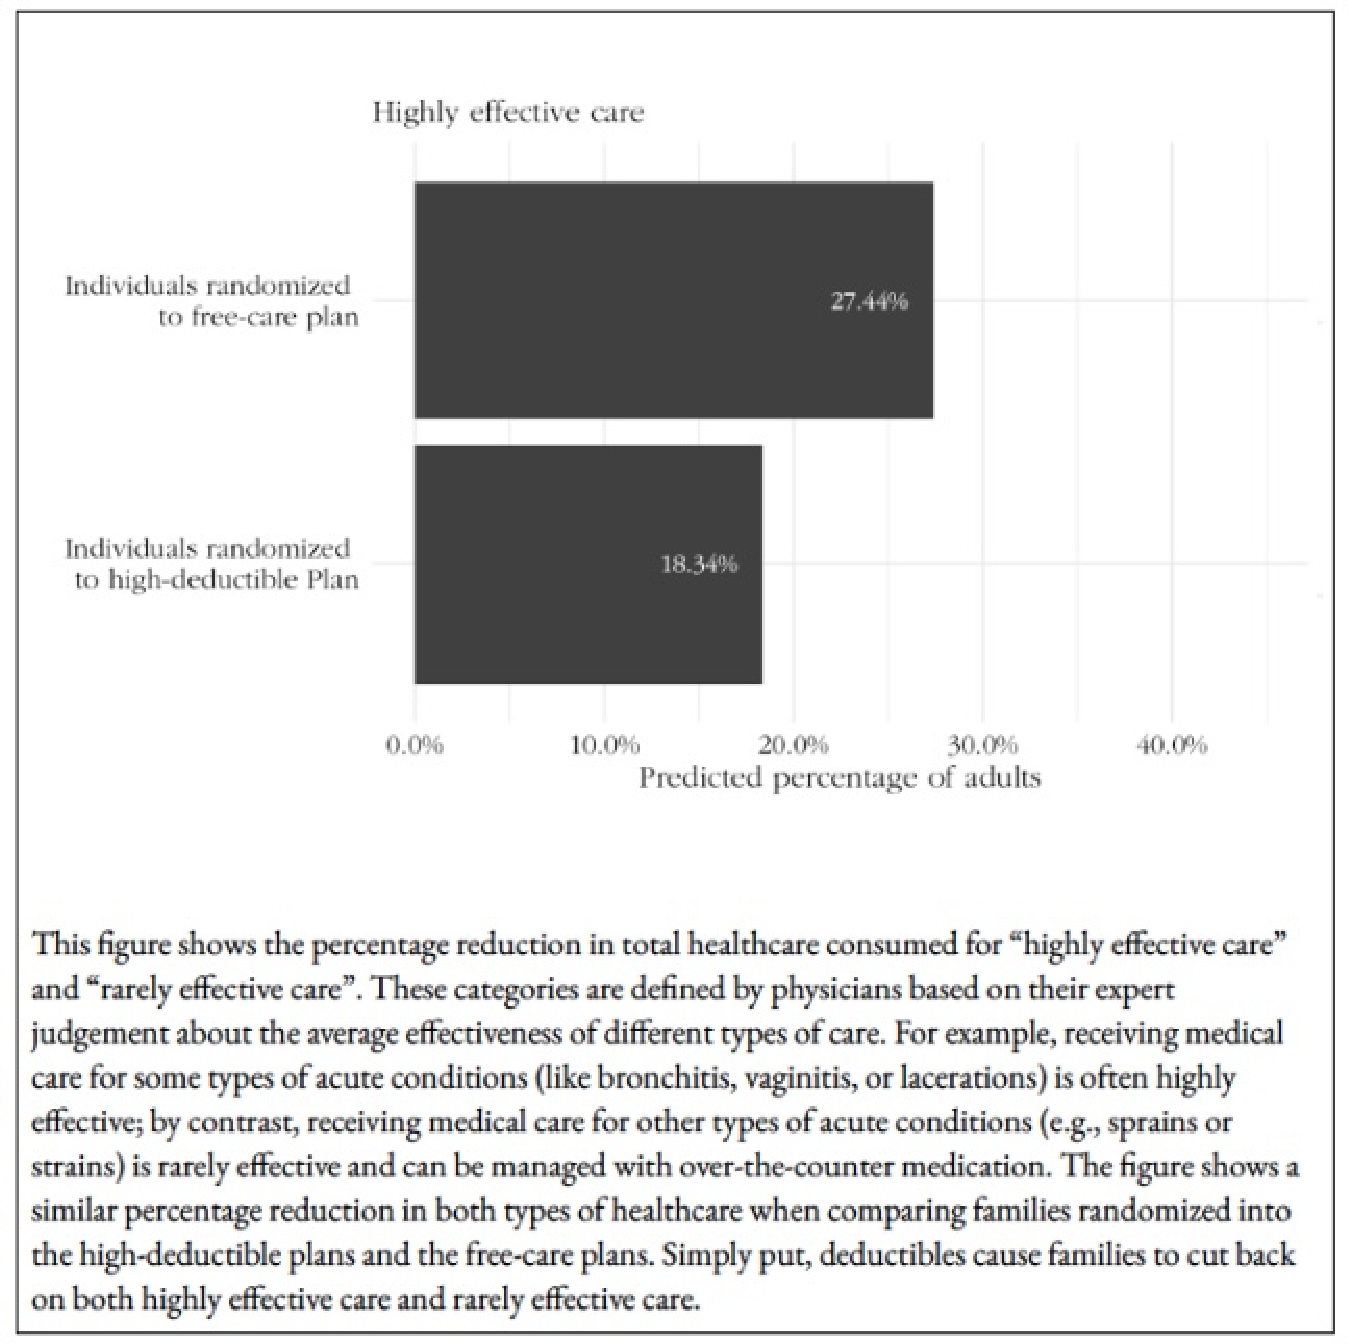
\includegraphics[width=0.45\textwidth]{input/RAND_effectivecare.pdf}
        \end{center}
        $\implies$ Which care is cut? Both ``rarely effective'' and ``effective'' care.
        }
\end{frame}
%---------------------------------------------------------------------
\begin{frame}{Impact on health?}

    \only<2>{
    \begin{center}
        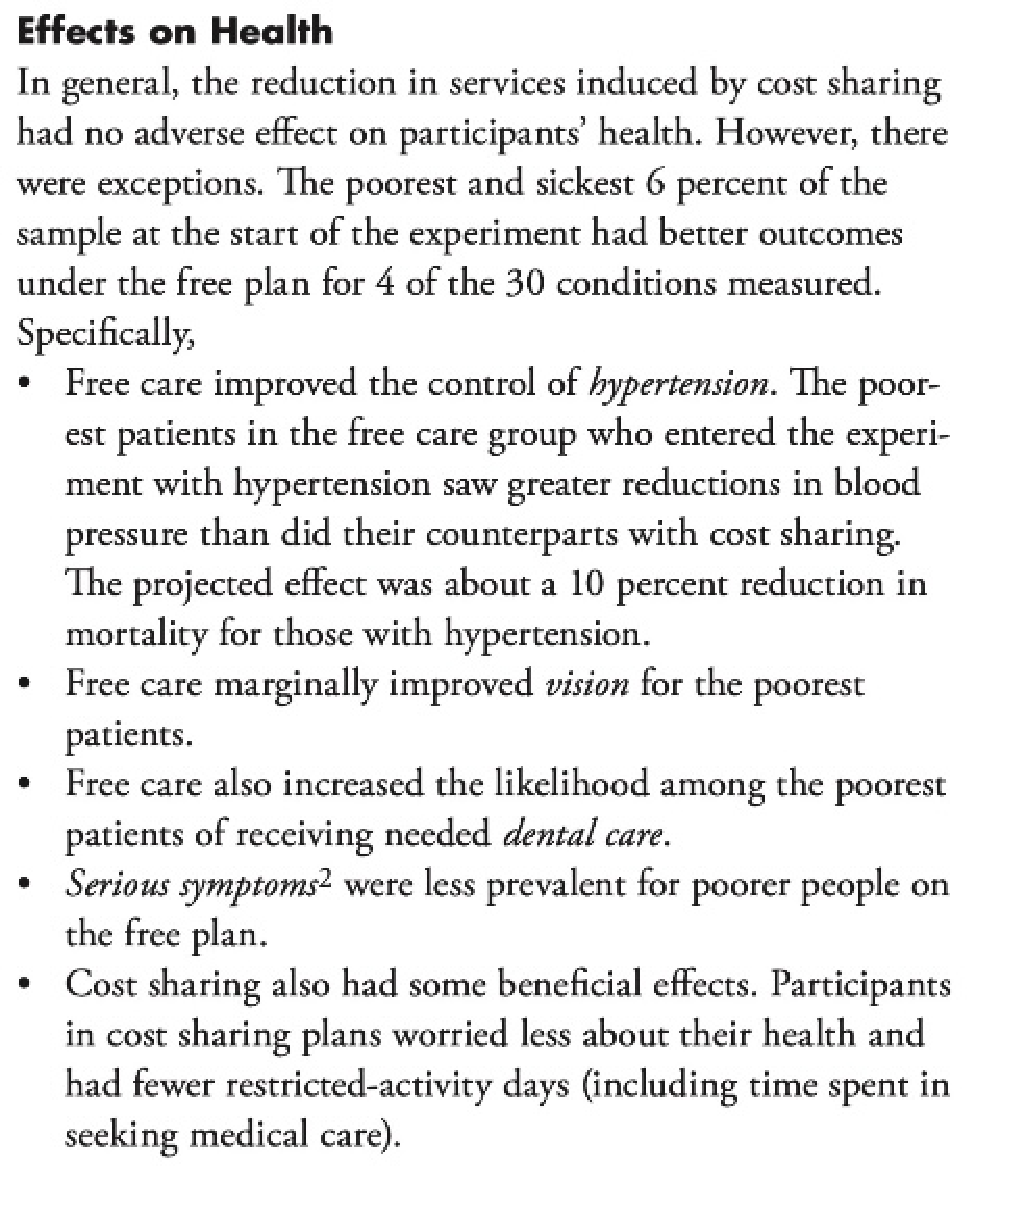
\includegraphics[width=0.4\textwidth]{input/RAND_effecthealth.pdf}
    \end{center}
    }

\end{frame}
%---------------------------------------------------------------------
\begin{frame}{The \newbold{RAND health insurance experiment}: conclusion}

    Main results:
    \begin{itemize}
        \item Healthcare demand slopes down (elasticity $\approx$ -0.2)
        \item Insurance increases the demand for healthcare
        \item Which care is cut: both ``effective'' and ``rarely effective'' care
        \item Impact on health? None on average but poor adults are hurt
    \end{itemize}
    \vspace{3mm}
  
        
    Legacy
        \begin{itemize}
            \item Largest and most expensive RCT in social science to date
            \item No impact on health: paved the way for cost-sharing (80s) and \textcolor{gray}{high-deductible} plans (2000s)
        \end{itemize}

\end{frame}
%---------------------------------------------------------------------
\begin{frame}{What is the impact of health insurance?}

    Insurance reduces the prices faced by patients\\
    $\rightarrow$ increases the demand for healthcare\\
    $\rightarrow$ increases healthcare utilization\\
    \vspace{5mm}

    A trade-off:
    \begin{itemize}
        \item Some healthcare is not very effective for some patients $\rightarrow$ more insurance $\rightarrow$ small gains and high costs
        \item Some healthcare is effective $\rightarrow$ more insurance $\rightarrow$ better health $\rightarrow$ could lead to less spending!
    \end{itemize}

\end{frame}
%---------------------------------------------------------------------
\begin{frame}{What is the impact of health insurance?}

    What do we want to know?
    \begin{align*}
        y_{i} = \pi_0 + \pi_1 \text{INSURANCE}_i + X'_{i} \pi_2 + \epsilon_{i}
    \end{align*}
    where
    \begin{itemize}
        \item $y_i$ is an outcome of interest for individual $i$ (e.g., healthcare utilization, health, financial health)
        \item $\text{INSURANCE}_i$ is whether $i$ has insurance
        \item $X_i$ are observables on individual $i$ (e.g., income, gender, age, etc.)
    \end{itemize}
    \vspace{2mm}

    Parameter of interest? \only<2>{{\color{red} $\pi_1$}}.
    
\end{frame}
%---------------------------------------------------------------------
\begin{frame}{What is the impact of health insurance?}

    What do we want to know?
    \begin{align*}
        y_{i} = \pi_0 + {\color{red} \pi_1} \text{INSURANCE}_i + X'_{i} \pi_2 + \epsilon_{i}
    \end{align*}
    \vspace{3mm}

    Problem? \only<2>{\newbold{Endogeneity of insurance}.\\
    This means that $\text{INSURANCE}_i$ is correlated with $\epsilon_i$:
    \begin{align*}
        cov(\text{INSURANCE}_i, \epsilon_i) \neq 0
    \end{align*}
    Thus OLS estimates of $\pi_1$ will be biased and inconsistent.
    \vspace{4mm}

    What do we do? \textit{We find some exogenous variation in insurance coverage.} How? Let's see this next week.}

    \only<1>{\vspace{35mm}}

\end{frame}
%---------------------------------------------------------------------
\begin{frame}{}
    \begin{center}
    \Large \textcolor{maroon}{Wrapping up}
    \end{center}
\end{frame}
%---------------------------------------------------------------------
\begin{frame}{What we covered today}
    \begin{itemize}
    \item Moral hazard: definitions
    \item Reminders on demand elasticity
    \item The RAND Health Insurance Experiment
\end{itemize}
\end{frame}
%---------------------------------------------------------------------
\begin{frame}{To next class}
\begin{itemize}
    \item \newbold{TO DO}
    \begin{enumerate}
        \item \newbold{Problem Set 2} due by \newbold{9:30am next Thursday 02/12}
        \item Review this class and past material $\implies$ \textit{questions on it?}
    \end{enumerate}
    \vspace{5mm}

    \item Program for next class
    \begin{itemize}
        \item The impact of health insurance
        \item Other ways to reduce moral hazard
    \end{itemize}
\end{itemize}
\end{frame}
%---------------------------------------------------------------------